\label{chap:method}
This chapter answers the second research question by presenting the Semantic-to-Metric agent. \ours instantiates the
factorization of \cref{eq:factor}: the VLM is its semantic sensor, and the agent owns all state and every decision.
\Cref{sec:method-principles} states the design principles, \cref{sec:method-overview} gives the complete loop, and
the following sections describe its parts in the order in which one step runs: the per-image questions
(\cref{sec:method-questions}), the metric hypothesis memory (\cref{sec:method-memory}), and search and control
(\cref{sec:method-control}). \Cref{sec:method-rgb,sec:method-stop} describe the RGB-only and explicit-stop variants.

\section{Design principles}
\label{sec:method-principles}
Three principles follow from the diagnosis of \cref{chap:diagnosis}.
\begin{enumerate}
\item \textbf{Ask only what the image can settle.} Every query to the VLM concerns the current frame, or a crop or tile
of it, and the target phrase. No query contains the action history, the map, or earlier answers, so every answer can
be checked against the image alone.
\item \textbf{Keep the state in metric form.} Where the target may be, which space is free, and which directions have
been looked at are stored as positions, evidence values, and grid cells, and are updated by explicit rules.
\item \textbf{Treat answers as evidence.} Because single answers are unreliable (\cref{sec:diag-probe}), no single
box decides the target. Evidence accumulates over distinct viewpoints and is withdrawn when an expected detection
does not appear.
\end{enumerate}
\Cref{tab:design-map} maps each part of \ours to the failure mode of \cref{sec:diag-state} that it addresses.

\begin{table}[htbp]
\centering\small
\caption{Parts of \ours and the diagnosed failure modes they address.}
\label{tab:design-map}
\begin{tabular*}{\linewidth}{@{\extracolsep{\fill}}lll@{}}
\toprule
Part & Section & Failure mode addressed\\
\midrule
Hypothesis memory with fusion & \cref{sec:method-memory} & lost after seen; acting on false boxes\\
Occupancy map and A* planner & \cref{sec:method-planning} & blocked by collisions\\
Look-around and exploration & \cref{sec:method-search} & target never seen (Long)\\
Crop check and tiled search & \cref{sec:method-questions} & weak or missed detections\\
Exhaustion on arrival & \cref{sec:method-commit} & committing to a look-alike\\
\bottomrule
\end{tabular*}
\end{table}

\section{Overview}
\label{sec:method-overview}
The belief $\mathcal{B}_t=(\mathcal{H}_t,M_t)$ of \ours consists of a list of target hypotheses $\mathcal{H}_t$ and an
occupancy map $M_t$. \Cref{fig:mech} shows one step as a flowchart, and \cref{alg:s2m} gives it as pseudocode.

\begin{figure}[htbp]
\centering
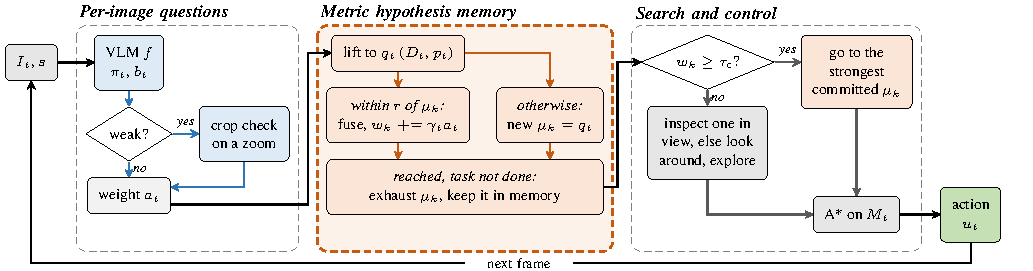
\includegraphics[width=\linewidth]{figures/fig_mech.pdf}
\caption[One step of \ours]{One step of \ours. The frozen VLM $f$ gives the presence $\pi_t$ and box $b_t$ of the
phrase $s$ on the frame $I_t$; a weak answer is checked on a crop or on tiles, which sets its weight $a_t$. The box is
lifted to a floor point $q_t$ with depth $D_t$ and pose $p_t$ and fused into a hypothesis $\mu_k$ within $r$, or
starts one; $\gamma_t<1$ discounts a repeated view, and a hypothesis that should be seen but is not loses $\lambda$ of
its evidence $w_k$. Above $\tau_c$ a hypothesis is committed, and the agent goes to $\mu_{k^\star}$; A* on the map
$M_t$ gives the action $u_t$.}
\label{fig:mech}
\end{figure}

\begin{algorithm}[htbp]
\caption{One step of \ours}
\label{alg:s2m}
\KwIn{frame $I_t$, depth $D_t$, pose $p_t$, last action flag $o_{t-1}$; target phrase $s$; belief $(\mathcal{H},M)$}
\KwOut{action $u_t$}
update $M$ with $D_t$ and $p_t$; mark the last move forbidden if $o_{t-1}=0$\;
$(\pi_t,b_t)\leftarrow$ presence and box queries of $f$ on $(I_t,s)$, in parallel\;
\If{$b_t\neq\varnothing$}{
  $a_t\leftarrow$ observation weight (\cref{eq:weight}), with a crop check if the answer is weak\;
  $q_t\leftarrow$ lift $b_t$ with $D_t$ and $p_t$ (\cref{eq:lift})\;
}
\If{no observation has $a_t\ge0.5$ and no hypothesis is committed}{
  add the crop-checked boxes of a $3{\times}3$ tiled search\;
}
\ForEach{observation $(q_t,a_t)$}{
  fuse into the first $\mu_k$ within $r$ (\cref{eq:fuse}), else create a new hypothesis $(q_t,a_t)$\;
}
lower every visible, undetected hypothesis by $\lambda$ (\cref{eq:neg}); remove those with $w_k\le-1$\;
\uIf{some hypothesis is committed ($w_k\ge\tau_c$, kept while $w_k\ge\tau_k$)}{
  $k^\star\leftarrow$ the committed hypothesis with the largest search index (\cref{eq:index})\;
  \lIf{the agent is within 0.9\,m of $\mu_{k^\star}$}{mark $k^\star$ exhausted and select again}
  \Return{the first action of A* from $p_t$ to $\mu_{k^\star}$ on $M$}\;
}
\uElseIf{the 360$^\circ$ look-around is incomplete}{\Return{a turn toward an unseen heading}\;}
\uElseIf{the strongest hypothesis has $w_k\ge0.35$}{\Return{the first action of A* toward it}\;}
\Else{\Return{the first action of A* toward the free cell 0.75--3\,m away that is farthest from all visited positions}\;}
\end{algorithm}

\section{Per-image questions}
\label{sec:method-questions}
\subsection{Target phrase}
At the start of an episode, one text-only query asks the VLM $f$ to rewrite the instruction $\ell$ into a target
phrase $s$. The reply names the most likely specific household object in one or two words, states whether the
instruction describes the object only by its appearance, and lists the appearance words. The phrase $s$ is the
category when the instruction names or implies one, and the appearance words when it describes only how the object
looks. The exact prompt is given in \cref{sec:appA-prompts}.

\subsection{Presence and box}
At every step, two queries about the current frame run in parallel. The presence query asks whether the image shows
$s$ and generates a single token. Its probability is read from the ten most likely first tokens,
\begin{equation}
\pi_t=\frac{P_f(\textit{yes}\mid I_t,s)}{P_f(\textit{yes}\mid I_t,s)+P_f(\textit{no}\mid I_t,s)},
\label{eq:presence}
\end{equation}
where the probabilities sum over the case variants of each answer, and $\pi_t=0.5$ if neither appears. The box query
asks for the bounding box of $s$ in a fixed JSON format, or an empty list if $s$ is not in the image; it returns a box
$b_t$ or none. Reading a probability instead of a yes/no answer gives a graded signal at the cost of one generated
token.

\subsection{Lifting}
\label{sec:method-lift}
A box with centre $c(b_t)=(u,v)$ is lifted with the median depth $\tilde d_t$ over its central half, that is, half
its width and half its height, which discards background pixels at the box border. With focal length $\varphi$ and
principal point $(u_0,v_0)$ of the pinhole camera, tilt $\phi_t$, and the forward and right unit vectors
$e_f(\theta_t),e_r(\theta_t)$ of the heading,
\begin{equation}
q_t=x_t+\tilde d_t\Big[\big(\cos\phi_t-\tfrac{v-v_0}{\varphi}\sin\phi_t\big)\,e_f(\theta_t)
+\tfrac{u-u_0}{\varphi}\,e_r(\theta_t)\Big],
\label{eq:lift}
\end{equation}
which is written $q_t=\Pi_{p_t}^{-1}(c(b_t),\tilde d_t)$. Lifts with $\tilde d_t>6$\,m are discarded. The same
back-projection, with the known camera height, labels each depth pixel as floor (height below 0.10\,m) or obstacle
(0.10--1.9\,m) and writes it into a 5\,cm occupancy grid $M_t$~\cite{elfes1989occupancy}.

\subsection{Observation weight and crop check}
A lifted box enters the memory with weight
\begin{equation}
a_t=\begin{cases}\pi_t & \text{if the target is named and } \pi_t\ge\tfrac12,\\
\pi^z_t & \text{otherwise, if } \pi^z_t\ge\tfrac12,\\
0.2\,\pi^z_t & \text{otherwise,}\end{cases}
\label{eq:weight}
\end{equation}
where $\pi^z_t$ is the presence probability of a \emph{crop check}: a square crop around the box with a side of 2.5
times the box's longer side, resized to 448\,px and queried with the presence question. The crop is queried only when
presence and box disagree or when the goal is appearance-only, so its extra cost is paid only where the evidence is
weak. A rejected crop does not delete the box; it enters with a small weight that later views can confirm or refute.

\subsection{Magnified search}
\label{sec:method-tiles}
Small or distant targets are often missed in the full frame. When a view yields no observation with $a_t\ge0.5$ and
no hypothesis is committed, the frame is split into $3{\times}3$ tiles with 20\% overlap, each upsampled to 448\,px and
queried for a box in parallel. Up to four distinct tile boxes are crop-checked, and those with $\pi^z\ge0.5$ enter the
memory. The tiled search runs at most once per view and spends VLM calls rather than environment steps.

\section{Metric hypothesis memory}
\label{sec:method-memory}
\subsection{Association and fusion}
Each hypothesis $k$ stores a floor position $\mu_k$, evidence $w_k$, and the poses $V_k$ from which it was observed.
An observation $(q_t,a_t)$ is associated with the first hypothesis within $r=0.5$\,m. If there is one,
\begin{equation}
\mu_k\leftarrow\frac{n_k\mu_k+q_t}{n_k+1},\qquad w_k\leftarrow w_k+\gamma_t\,a_t ,
\label{eq:fuse}
\end{equation}
with $n_k$ the number of fused observations; otherwise a new hypothesis $(\mu,w)=(q_t,a_t)$ is created. The
discount is $\gamma_t=0.25$ if some $v\in V_k$ has the heading of $p_t$ and a position within 0.2\,m of it, and
$\gamma_t=1$ otherwise.

The discount is the key design choice of the memory. Two answers from the same viewpoint are not independent: the
model sees nearly the same image and tends to repeat itself, including its errors. Through $\gamma_t$, evidence grows
with the number of distinct viewpoints rather than with the number of frames, so a look-alike that the model boxes
repeatedly from one place cannot accumulate the evidence of a target confirmed from several places.

\subsection{Negative evidence}
\label{sec:method-neg}
A hypothesis that the current frame should show but that receives no detection loses evidence:
\begin{equation}
\begin{gathered}
w_k\leftarrow w_k-\lambda\,\mathbb{1}\big[\mathrm{vis}_t(\mu_k)\big],\\
\mathrm{vis}_t(\mu)\Leftrightarrow \bar u\in\Omega,\ \ d\le6\,\text{m},\ \ D_t(\bar u)+0.3\ge d,
\end{gathered}
\label{eq:neg}
\end{equation}
for every hypothesis without a detection within $r$, where $(\bar u,d)=\Pi_{p_t}(\mu)$ are its projected pixel and
planar depth, $\Omega$ is the image shrunk by 20\,px, and $\lambda=0.4$. The last condition rules out occlusion: a
hypothesis behind a nearer surface is not expected to be seen. Hypotheses with $w_k\le-1$ are removed. Absence
outside the view is never counted, so turning away from a hypothesis does not erase it.

\subsection{Commitment, hysteresis, and exhaustion}
\label{sec:method-commit}
The agent commits to a hypothesis once $w_k\ge\tau_c=0.8$ and keeps it while $w_k\ge\tau_k=0.4$. The hysteresis
prevents one missed detection from abandoning a well-supported target. When the agent stands within 0.9\,m of a
committed hypothesis and the episode continues, which on EB-Navigation means that it is not the target, the
hypothesis is marked exhausted. It stays in memory, so later detections of the same look-alike merge into it instead
of creating a new target.

\section{Search and control}
\label{sec:method-control}
\subsection{Selection among committed hypotheses}
Among the committed hypotheses $\mathcal{C}_t$ the agent visits
\begin{equation}
k^\star=\arg\max_{k\in\mathcal{C}_t}\ \frac{1-e^{-w_k}}{c_k+1},\qquad c_k=\frac{\lVert\mu_k-x_t\rVert}{0.25\,\text{m}} .
\label{eq:index}
\end{equation}
The numerator maps the evidence to the probability of at least one detection under a Poisson model with mean $w_k$,
and the denominator counts the steps to reach and check $\mu_k$. For locations with fixed inspection costs,
inspecting in decreasing order of this probability-to-cost ratio is optimal~\cite{kadane1977optimal}; \ours applies
the rule greedily and recomputes the cost from the current position at every step. The index reduces to nearest-first
for equal evidence and to strongest-first for equal cost.

\subsection{Search without a committed target}
\label{sec:method-search}
With nothing committed, the agent first completes a 360$^\circ$ look-around by turning toward headings it has not yet
observed. It then approaches the strongest hypothesis if $w_k\ge0.35$, so that a weak detection can be confirmed or
refuted from closer. Otherwise it explores: it moves to the observed free cell 0.75--3\,m away that is farthest from
all positions it has visited, and repeats the look-around on arrival while enough steps remain. This rule is a
simple form of frontier exploration~\cite{yamauchi1997frontier} that never queries the model.

\subsection{Planning}
\label{sec:method-planning}
Actions come from A*~\cite{hart1968astar} over (position, heading) states on $M_t$, whose edges are the benchmark's
translations and turns. An edge costs 1 plus 0.15 for each of four sampled points on it that is unobserved, which
prefers known free space without forbidding unexplored space. Edges through obstacles inflated by the agent radius of
0.2\,m are removed. If the resulting path cannot end within 0.85\,m of the goal, the planner tries again with a
tighter inflation of 0.1\,m, which lets the agent pass narrow gaps between furniture, and keeps the better of the two
plans. A goal counts as reached within 0.55\,m.

A move that the simulator rejects is written into the map as a blocked segment, so the planner never repeats it. The
agent follows its current plan step by step and replans when the target estimate moves by more than 0.3\,m, when the
last action ended more than 0.12\,m from its expected position (because of grid snapping or a collision), or when
the next move has become invalid on the updated map. When the agent stands next to a committed hypothesis but no
move brings it closer, it takes the single move that best reduces the distance, which resolves the last centimetres
that the 0.25\,m action grid cannot plan.

\section{A worked example}
\label{sec:method-example}
\Cref{tab:trace} follows the memory of \ours through the Long-horizon test episode of \cref{fig:arch}, in which
the target is an alarm clock behind the agent. In the first two steps the agent turns and sees nothing ($\pi_t\approx0$).
At step 2 the alarm clock enters the view; the box is lifted and creates a hypothesis whose evidence $0.82$ already
exceeds $\tau_c$, so the agent commits and starts to approach. The evidence then grows with each new viewpoint. At
steps 5 and 8 the full-frame presence answer is low although a box is returned, the crop check confirms the target,
and the evidence increases by the crop's presence. At step 7 the model boxes a look-alike instead, the target is in view
but not detected, and negative evidence lowers the target by $\lambda=0.4$; the hysteresis keeps the commitment. At
step 9 the crop check rejects the box, so the step adds no evidence. Two look-alikes appear briefly with weights
below 0.1; each loses $\lambda$ at every following view in which it is visible but not detected, and neither ever
comes close to commitment. The episode ends successfully at step
\tTraceSteps{} with the target hypothesis at $w=\tTraceFinalW$.

\begin{table}[htbp]
\centering\small
\caption[Evidence of every hypothesis in one episode]{Evidence of every hypothesis of \ours in the Long-horizon test
episode of \cref{fig:arch} (Qwen3-VL-4B, target: \tTraceTarget). Observation: what the box query returned; $\pi_t$:
full-frame presence; $\pi^z_t$: presence on the crop; $a_t$: weight of the observation (\cref{eq:weight}); $w$:
evidence after the step; Action: the action taken. Bold: the target hypothesis is committed ($w\ge\tau_c$).}
\label{tab:trace}
\begin{tabular*}{\linewidth}{@{\extracolsep{\fill}}rlcccrll@{}}
\toprule
Step & Observation & $\pi_t$ & $\pi^z_t$ & $a_t$ & $w$ (target) & $w$ (look-alikes) & Action\\
\midrule
0 & no box & 0.00 & not asked & 0 & none & none & turn right\\
1 & no box & 0.00 & not asked & 0 & none & none & turn right\\
2 & box on target & 0.78 & not asked & 0.78 & 0.78 & none & forward\\
3 & box on target & 1.00 & not asked & 1.00 & \textbf{1.78} & none & forward\\
4 & box on target & 0.50 & not asked & 0.50 & \textbf{2.28} & none & forward\\
5 & box on target & 0.01 & 1.00 & 1.00 & \textbf{3.28} & none & forward\\
6 & box on target & 0.91 & not asked & 0.90 & \textbf{4.18} & none & forward\\
7 & box on look-alike & 0.00 & 0.32 & 0.06 & \textbf{4.18} & 0.06 & forward\\
8 & box on target & 0.38 & 1.00 & 1.00 & \textbf{5.18} & 0.06 & forward\\
9 & box, rejected & 0.27 & 0.08 & 0 & \textbf{5.18} & 0.06 & right\\
10 & box on target & 0.94 & not asked & 0.94 & \textbf{6.12} & 0.06 & forward\\
11 & box on look-alike & 0.15 & 0.88 & 0.88 & \textbf{6.12} & 0.95 & right\\
12 & box on target & 0.99 & not asked & 0.99 & \textbf{7.11} & 0.95 & right\\
13 & box on target & 0.99 & not asked & 0.99 & \textbf{8.10} & 0.95 & forward\\
\bottomrule
\end{tabular*}

\end{table}

The example shows the three mechanisms of the memory at work. Fusion turns a sequence of individually uncertain
answers into a hypothesis with high evidence. Negative evidence removes the look-alikes without ever committing to
them. Hysteresis keeps the agent on its target through one missed detection.

\section{Choice of parameters}
\label{sec:method-params}
The parameters of \ours (\cref{tab:s-params}) follow from the geometry of the task and were set on the development
split. The association radius $r=0.5$\,m is half the success radius, so two detections of one object fall into one
hypothesis while two objects on different pieces of furniture stay apart. The commit threshold $\tau_c=0.8$ is
reached by one confident answer from a named target ($\pi_t\ge0.8$) or by two moderate answers from different
viewpoints, and the keep threshold $\tau_k=0.4$ tolerates one missed detection, since one negative update subtracts
$\lambda=0.4$. The repeated-view discount $\gamma=0.25$ allows four looks from the same place to add as much as one
look from a new place. The removal threshold $w_k\le-1$ requires several unexplained misses before a hypothesis is
forgotten, so a target that was briefly occluded survives.

\section{Operating without a depth sensor}
\label{sec:method-rgb}
\subsection{Per-frame ground-plane scale}
Monocular metric depth networks err mostly by a frame-dependent scale. Let $\hat D_t$ be the raw prediction and
$\kappa(v)=\sin\phi_t+\frac{v-v_0}{\varphi}\cos\phi_t$ the downward component of the ray through row $v$ per unit of
planar depth. A pixel on the floor satisfies $\sigma\hat D_t(u,v)\,\kappa(v)=h$ for the camera height $h$, and an
object standing on the floor gives a larger $\sigma$. Over the pixels $\mathcal{F}_t$ whose rays point at least
15$^\circ$ below the horizontal, \ours takes the mode
\begin{equation}
\sigma_t=\operatorname*{mode}_{(u,v)\in\mathcal{F}_t}\ \frac{h}{\hat D_t(u,v)\,\kappa(v)},\qquad D_t=\sigma_t\,\hat D_t ,
\label{eq:floorscale}
\end{equation}
with the mode taken over values in $[\bar\sigma/1.33,\,1.33\,\bar\sigma]$, where $\bar\sigma$ is one global scale
fitted on development frames. It keeps $\bar\sigma$ when fewer than 10\% of the pixels in $\mathcal{F}_t$ fall in this
window. This is the ground-plane constraint of monocular visual odometry~\cite{song2014robust} applied to every frame.

\subsection{Pose from the executed actions}
Without simulator pose, the agent integrates its own executed actions,
\begin{equation}
\hat x_{t+1}=\hat x_t+0.25\,o_t\big(\alpha_f e_f(\hat\theta_t)+\alpha_r e_r(\hat\theta_t)\big),
\label{eq:deadreckon}
\end{equation}
with $(\alpha_f,\alpha_r)\in\{(\pm1,0),(0,\pm1)\}$ the translation of $u_t$; heading and tilt advance by the turn or
tilt of $u_t$ when $o_t=1$. The RGB-only configuration uses \cref{eq:floorscale,eq:deadreckon} together and has no
access to the simulator's depth or pose.

\section{Explicit stopping on RoboTHOR}
\label{sec:method-stop}
EB-Navigation ends an episode on success, whereas RoboTHOR requires a Stop action. There the agent stops only when it
is within 0.9\,m of a committed hypothesis, has turned within 20$^\circ$ of it and tilted it into view, and a fresh
presence query exceeds 0.5; otherwise the hypothesis is exhausted. Because RoboTHOR episodes last up to 500 steps,
negative evidence counts only within 3\,m and once per view, and exploration goes to the nearest frontier. These are
the only changes between the two benchmarks.

\section{Information access and implementation}
\label{sec:method-impl}
The VLM sees the current image, a crop or tile of it, and $s$; the controller sees depth, pose, and action success,
but never the target position or any simulator metadata. \ours is implemented in Python on top of the benchmark's
environment; the VLM queries are sent to a local vLLM server, and the presence and box queries of a step, as well as
the queries of the tiles, run in parallel. All parameters are listed in \cref{tab:s-params} and were fixed on the
development split.

\section{Summary}
\ours replaces the model's role, not the model. The VLM answers two questions per frame, and a metric memory, a
search rule, and a planner turn these answers into actions. The memory is built for a generative sensor whose single
answers are unreliable: evidence grows only with distinct viewpoints and is withdrawn when an expected detection does
not appear. The next chapter tests whether this design removes the failures diagnosed in \cref{chap:diagnosis}.
